% This document provides the style to be used for a MSc Thesis at the
% Parallel and Distributed Systems group
\documentclass[11pt,twoside,a4paper,openright]{report}

% use babel for proper hyphenation
\usepackage[british]{babel}
\usepackage{graphicx}
\graphicspath{{../figures/}}
\usepackage{url}
\usepackage{algpseudocode} 
\usepackage{amsmath}
\usepackage{amssymb}
\usepackage{amsthm}
\usepackage{cleveref}
\usepackage{subcaption}
\usepackage{rotating}

\DeclareMathOperator*{\argmin}{arg\,min}
\newtheorem{theorem}{Theorem}
\newtheorem{corollary}{Corollary}
\newtheorem{lemma}{Lemma}

\newcommand{\Cons}{\mathcal{C}}
\newcommand{\Pideal}{\Pi_{\text{ideal}}}
\newcommand{\Preal}{\Pi_{\text{real}}}
\newcommand{\Fideal}{\mathcal{F}_{\text{ideal}}}

%use this command when you want the next content to appear on an odd page
\newcommand{\clearemptydoublepage}{
    \newpage{\pagestyle{empty}
    \cleardoublepage}
}

\begin{document}

%%%%%%%%%%%%%%%%%%%%%%%%%%%%%%%%%%%%%%%%%%%%%%%%%%%%%%%%%%%%%%%%%%%%%%%%%%%%%%%
\hoffset=1.63cm
\oddsidemargin=0in
\evensidemargin=0in
\textwidth=5in

%%%%%%%%%%%%%%%%%%%%%%%%%%%%%%%%%%%%%%%%%%%%%%%%%%%%%%%%%%%%%%%%%%%%%%%%%%%%%%%
\parindent=1em

\pagestyle{empty}

% FRONTCOVER
\begin{titlepage}

\null\vfill

\begin{center}
\LARGE{TODO TITLE}
\end{center}

\vspace{1.5cm}

\begin{center}
Kelong Cong
\end{center}

\vfill

\begin{figure}[!b]
\centering

\includegraphics[width={0.6\textwidth}]{logo}
\end{figure}

\vspace{2.0cm}

\end{titlepage}



% EMPTY PAGE
\cleardoublepage

\pagestyle{plain}

% TITLE PAGE: page i (hidden)
\begin{titlepage}
\begin{center}

\includegraphics[height=4cm]{figures/logo}\\
%\LARGE
%Delft University of Technology \\
\large
Faculty Electrical Engineering, Mathematics and Computer Science

\vspace*{12cm}

\setlength{\TPHorizModule}{1mm}
\setlength{\TPVertModule}{\TPHorizModule}
% Set the Paragraph Indent to zero, so the first line is not Indented
% Back-up the current value so it can be put back at the end of the title page
\newlength{\backupparindent}
\setlength{\backupparindent}{\parindent}
\setlength{\parindent}{0mm}			
% Begins a textbox at 72 mm from the left of the edge of the paper and 89 mm from the top
% The width of the textbox is 95 mm (167 - 72 mm)
% The height of the box cannot be defined, so it is your task to keep the text not too long
\begin{textblock}{95}(62,89)
    \vspace*{7mm}
    \huge
    \textbf{\doctitle \\}
    \Large
    \vspace*{3mm}
    \textit{\docsubtitle}\\
    \vspace*{10mm}
    \Large
    \me\\
\end{textblock}

\large
Supervisors:\\
\begin{tabular}{rl}
    \firstCommitteeMember\\
    \secondCommitteeMember\\
    \thirdCommitteeMember\\
\end{tabular}

\vfill
\version

\vfill
%\docdate \\
\large
Delft, \monthYear\\

% Put the Paragraph Indent back to its original value
\setlength{\parindent}{\backupparindent}
\end{center}
\end{titlepage} 


% GRADUATION DATA AND ABSTRACT: pages ii and iii (hidden)
%De aankondiging bevat de spreker, titel, plaats, datum en tijd, samenstelling van de afstudeercommissie en een korte samenvatting (maximaal 25 regels).
\thispagestyle{empty}

\noindent \textbf{Author}\\
\begin{tabular}{l}
Kelong Cong\\
\\
\end{tabular}\\
\noindent \textbf{Title}\\
\begin{tabular}{l}
A Blockchain Consensus Protocol With Horizontal Scalability\\
\\
\end{tabular}\\
\noindent \textbf{MSc presentation}\\
\begin{tabular}{l}
% <MM> DD, YYYY (like \today)
31st August 2017\\
\\
\end{tabular}

\vspace{1.1cm}

\noindent \textbf{Graduation Committee}\\
\begin{tabular}{ll}
% The order of listing the names: Graduation prof, supervisor(s), others ordered by title + alphabetical
%examples:
Prof. dr. ir. D. H. J. Epema            & Delft University of Technology \\
Dr. ir. J. A. Pouwelse                  & Delft University of Technology \\
Dr. Z. Erkin                            & Delft University of Technology \\
\end{tabular}

\begin{abstract}
% what's the problem?
Blockchain systems have the potential to decentralise many traditionally centralised systems.
However, scalability remains a key challenge.
Without a horizontally scalable solution, blockchain systems remain unsuitable for ubiquitous use.
% what's the solution?
We design a novel blockchain system called \textsc{Checo}.
Each node in our system maintains a personal hash chain,
which only stores transactions that the node is involved in.
A consensus is reached on special blocks called checkpoint blocks rather than on all the transactions.
Checkpoint blocks are effectively a hash pointer to the personal hash chains,
thus a single checkpoint block may represent a large set of transactions.
The consensus protocol does not imply transaction validity.
Hence we introduce a validation protocol which allows nodes to verify that the transactions are correctly recorded,
meaning that consensus on transactions is achieved indirectly via checkpoint blocks.
% how good is the solution?
We evaluate \textsc{Checo} analytically and experimentally.
Our results show a strong indication of horizontal scalability even in the worst case,
where every transaction is made with a randomly selected node.
\end{abstract}

\clearpage



\pagenumbering{roman}
\setcounter{page}{4}

% EMPTY PAGE: page iv
\cleardoublepage

% OPTIONAL QUOTATION: page v
%\pagestyle{empty}

\null\vfill

\begin{center}
\emph{``TODO QUOTE''} -- TODO QUOTED PERSON
\end{center}

\vspace{10cm}

\clearpage


% EMPTY PAGE: page vi
%\cleardoublepage

% PREFACE: page v
\chapter*{Preface}
\addcontentsline{toc}{chapter}{Preface}
TODO MOTIVATION FOR RESEARCH TOPIC

\vspace{1\baselineskip}

\noindent
TODO ACKNOWLEDGEMENTS

\vspace{1\baselineskip}

\noindent
TODO AUTHOR

\vspace{1\baselineskip}

\noindent
Delft, The Netherlands

\noindent
\today

% EMPTY PAGE: page vi
\cleardoublepage

% TABLE OF CONTENTS: starting at page vii
\tableofcontents

\cleardoublepage

\pagenumbering{arabic}
\setcounter{page}{1}

This is a story about a scalable blockchain framework and Byzantine
generals\dots

%%% Local Variables:
%%% mode: latex
%%% TeX-master: "../thesis"
%%% End:
\clearemptydoublepage

\chapter{System Architecture}
\label{ch:model}

The primary goal guiding our design is scalability.
As mentioned in the Introduction, having a scalable blockchain system while still keeping global consensus
allows the system to be ubiquitous and realise the full potential of blockchain.

The secondary goal is to design an application neutral system.
In particular, it should act as a framework that provides the building blocks of blockchain based applications.
Application developers using the framework should be able to create any application they wish.
Further, we do not impose on a consensus algorithm, as long as it satisfies the properties of atomic broadcast which we describe in~\Cref{sec:overview-cons}.

Due to the nature of our system, we do not explicitly address the Sybil attack~\cite{douceur2002sybil}.
Sybil defence mechanism always require some form of reputation score from the application.
For example, social network based Sybil defence mechanims use graph structure of real-world relationships~\cite{yu2006sybilguard}.
Online marketplaces such as Amazon use the rating of buyer and sellers.
Thus it is not possible to design a Sybil defence mechanism with a a application neutral framework.
On the other hand, our system also has no restrictions on the Sybil defence technique
and application designers can pick the best mechanism for their application.

The third and final goal is security.
Our system should be unaffected in the presence of powerful adversaries.
Security is often difficult to verify, especially when it is not formalised, therefore we require our design to be provably secure.
To summarise, our system design is designed with the following goals in mind.
\begin{itemize}
    \item Application neutrality,
    \item scalability and
    \item security.
\end{itemize}

We begin the chapter with an intuitive overview of the architecture in \Cref{sec:system-overview}.
Next, we give the formal description, starting with the model and assumptions in \Cref{sec:model-assumptions}.
Then, the three protocols which make up the complete system,
namely consensus protocol (\Cref{sec:cons-protocol}), transaction protocol (\Cref{sec:tx-protocol}) and validation protocol (\Cref{sec:vd-protocol}).
Finally, the possible extensions are described in \Cref{sec:protocol-extensions}.


\section{System Overview}
\label{sec:system-overview}
The system consist of one data structure---Extended TrustChain,
and three protocols---consensus protocol, transaction protocol and validation protocol.
We first describe each component individually and then explain how they fit together in \Cref{sec:combined-protocol}.

\subsection{Extended TrustChain}
Extended TrustChain naturally builds on top of TrustChain, thus we first describe the standard TrustChain.
Our description has minor differences compared to the description in~\cite{trustchain}.
This is to help with the description of the extended TrustChain.
However, the two descriptions are functionally the same.

\subsubsection*{Standard TrustChain}
In TrustChain, every node has a ``personal'' chain. 
Initially, the chain only contains a genesis block.
When a node wishes to add a new transaction (TX), a new TX block is generated and is appended to the chain.
A TX block must have a valid hash pointer pointing to the previous block
and a reference\footnote{This is different from the original TrustChain definition found in~\cite{trustchain}.
In there, a TX block has two outgoing edges which are hash pointers to the two parties involved in the transaction.
This work uses one outgoing edge and a reference.} to its \emph{pair}.
As a result, a single transaction generates two TX blocks, one on each party's chain.
An example of is shown in \Cref{fig:trustchain-bad}.

\begin{figure}
    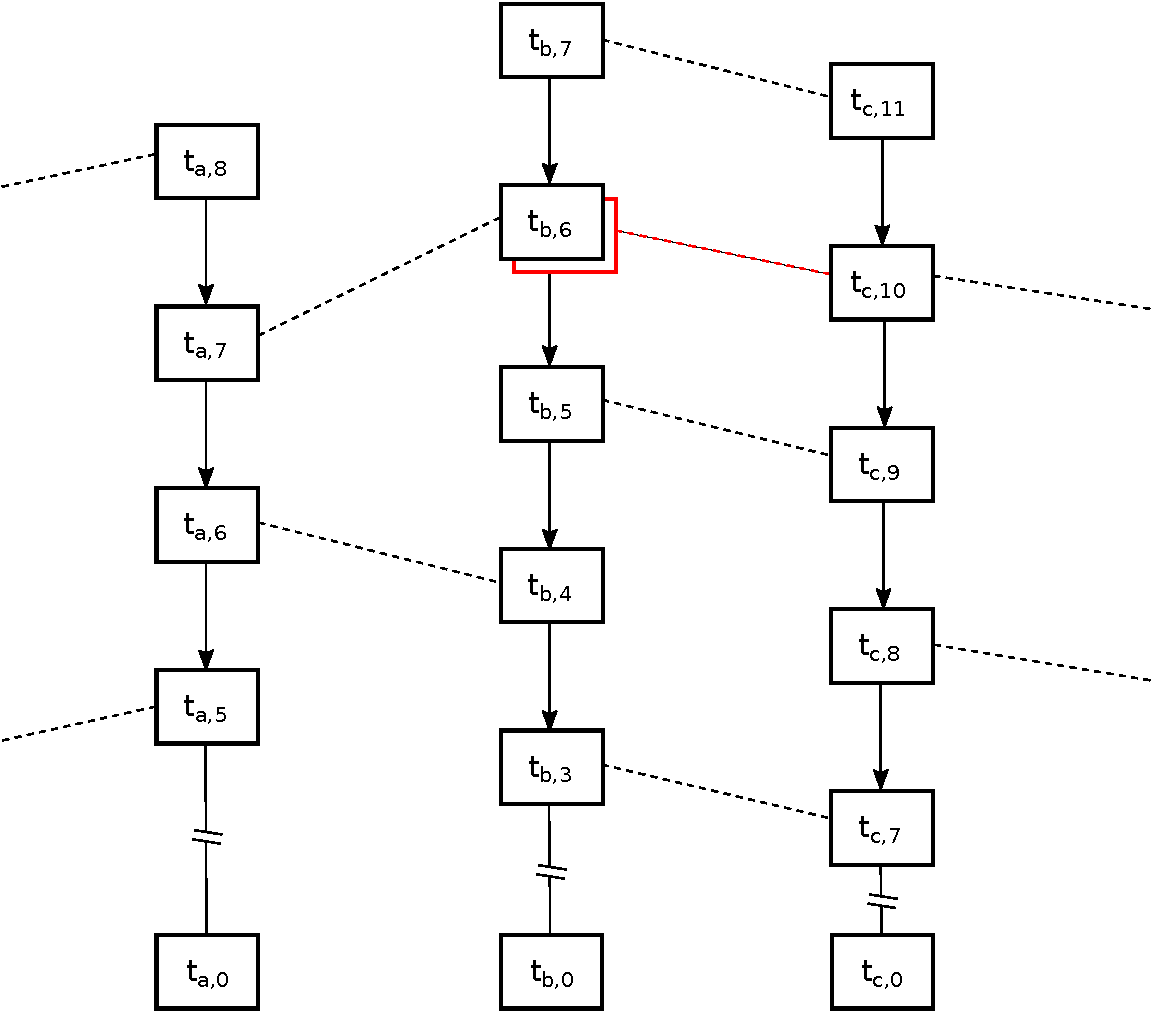
\includegraphics[width=0.9\textwidth]{trustchain-bad}
    \centering
    \caption{Every block is denoted by $t_{i,j}$, where $i$ is the node ID and $j$ is the sequence number of the block.
    Thus we have three nodes and three corresponding chains in this example.
    The arrows represent hash pointers and the dotted lines represent references.
    The blocks at the ends of one dotted line are pairs of each other.
    The red block after $t_{b, 5}$ indicate a fork.}
    \label{fig:trustchain-bad}
\end{figure}

If every node follows the rules of TrustChain and we only consider hash pointers,
then the chain effectively forms a singly linked list.
However, if a node violates the rules, then a \emph{fork} may happen.
That is, there may be more than one TX block with a hash pointer pointing back to the same block.
In \Cref{fig:trustchain-bad}, node $b$ (in the middle chain) created two TX blocks that both point to $t_{b, 5}$.
If this is a ledger system it can be seen as a double spend, where the currency accumulated up until $t_{b, 5}$ are spent twice.

\subsubsection*{Extended TrustChain}
We are now ready to explain the Extended TrustChain, which we abbreviate to ETC.
In ETC, we introduce a new type of block---checkpoint (CP) block.
In contract to TX blocks, CP blocks do not store transactions or contain references.
Their purpose is to capture the state of the chain and the state of the whole system.
In particular, the state of the chain is captured with a hash pointer.
The state of the whole system is captured in the content of the CP block,
namely as a digest of the latest \emph{consensus result} which we explain in \Cref{sec:overview-cons}.
A visual representation is shown in \Cref{fig:trustchain-bad-cp}.

\begin{figure}
    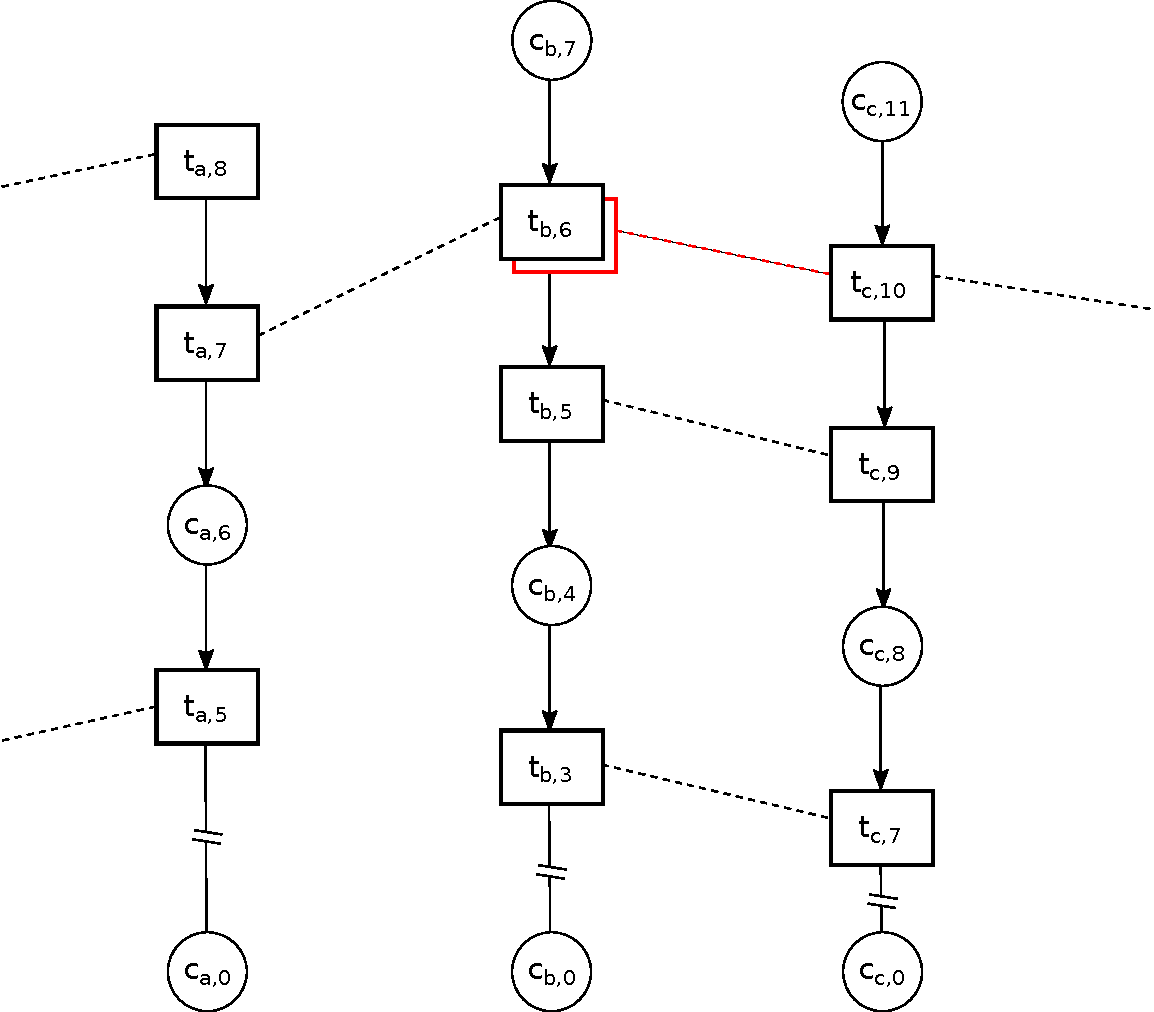
\includegraphics[width=0.9\textwidth]{trustchain-bad-cp}
    \centering
    \caption{The circles represent CP blocks,
    they also have hash pointers (arrow) but do not have references (dotted line).
    Note that the sequence number counter do not change, it is shared with TX blocks.}
    \label{fig:trustchain-bad-cp}
\end{figure}

\subsection{Consensus Protocol}\label{sec:overview-cons}

% The consensus protocol uses an existing Byzantine consensus algorithm (explained in detail in \Cref{sec:xyz}) and runs it continuously in rounds.
The consensus protocol can be seen as a technique of running infinitly many rounds of some 
Byzantine consensus algorithm\footnote{More accuratly it is ACS or asynchronous subset consensus, we describe ACS in \Cref{sec:acs}.},
starting a new execution immediately after the previous one is completed.
This is necessary because blockchain systems always need to reach consensus on new values, or CP blocks in our case.

The high message complexity of Byzantine consensus algorithms prohibits us from running it on a large network.
Thus, for every round, we randomly select some node---called facilitators---to collect CP blocks and use them as the proposal.
The facilitators are elected using a \emph{luck value}, which is computed using $H(\C_r || pk_i)$,
where $\C_r$ is the consensus result (a set of CP blocks) in round $r$ and $pk_i$ is the public key of $i$.
Intuitively, the election is guaranteed to be random 
because the output of a cryptographically secure hash function is unpredictable and $\C_r$ cannot be determined in advance.

A visual explaination can be found in \Cref{app:consensus-example},
it walks through the steps needed for a node to be selected as a facilitator.

\subsection{Transaction and Validation}
The TX protocol is a simple request and response protocol.
The nodes exchange one round of messages and create new TX blocks on their respective chains.
Thus, as we mentioned before, one transaction should result in two TX blocks.

The consensus and transaction protocol by themselves do not provide a mechanism to detect forks or other forms of tamperaing.
Thus we need a validation protocol to counteract malicious behaviour.
When a node wish to validate one of its TX, it asks the counterparty for the \emph{fragment} of the TX.
A fragment of a TX is a section of the chain beginning and ending with CP blocks that contains the TX.
Upon the counterparty's response, the node checks that the CP blocks are in consensus, the hash pointers are valid and his TX is actually in the fragment.
The TX is valid if these conditions are satisfied.
Intuitively, this works because it is hard (because hash collision is hard)
 to create a different chain that begins and ends with the same two CP blocks but with a different middle section.


\subsection{Combined Protocol}
\label{sec:combined-protocol}
The final protocol is essentially the concurrent composition of the three aforementioned protocols,
all making use the Extended TrustChain data structure.

Our subprotocol design gives us the highly desireable non-blocking property.
In particular, we do not need to ``freeze'' the state of the chain for some communication to complete in order to create a block.
For instance, a node may start the consensus protocol, and while it is running, the node may still perform transactions.
By the time the consensus protocol is done, the new CP block is added to whatever the state that the chain is in.
It is not necessary to keep the chain immutable while the consensus protocol is running.

\section{Model and Assumptions}
\label{sec:model-assumptions}

For notational clarify, we use the following convention (adapted from~\cite{miller2016honey}) throughout this work.
\begin{itemize}
\item Lower case (e.g. $x$) denotes a scalar object or a tuple.
\item Upper case (e.g. $X$) denotes a set or a constant.
\item Sans serif (e.g. $\textsf{fn}(\cdot)$) denotes a function.
\item Typewrite (e.g. $\texttt{ack}$) denotes message type.
\end{itemize}
Further, we use $a || b$ to dedote concatination of the binary representations of $a$ and $b$.

We assume a distributed network where nodes are fully connected,
the channels are reliable\footnote{
    Reliability can be achieved in unreliable networks by resending messages or using some error correction code.
},
but messages may be re-ordered and delayed by at most some time $\Delta$,
this is sometimes known as a $\Delta$-synchronous network.
We assume there exist a Public Key Infrastructure (PKI), and nodes are identified by their unique and permanent public key.
Finally, we use the random oracle model, i.e. calls to the random oracle are denoted by $\textsf{H}: \{0, 1\}^* \rightarrow \{0, 1\}^\lambda$,
where $\{0, 1\}^*$ denotes the space of finite binary strings and $\lambda$ is the security parameter~\cite{bellare1993random}.

In our model we consider $N$ nodes, which is the population size.
$n$ of them are facilitators, $t$ out of $n$ are malicious and the inequality
$n \ge 3t + 1$ must hold.

We use a restricted version of the adaptive corruption model.
The first restriction is that corrupted node can only change across rounds.
That is, if a round has started, the corrupted nodes cannot changed until the next round.
The second restriction is that the adversary, presumably controlling all the corrupted nodes, is forgetful.
Namely the adversary may learn the internal state such as the private key of a corrupted node,
but if the node recovers, then the adversary must forget the private key.
Otherwise the adversary can eventually learn all the private keys and sabotage the system.
Finally, we assume computational security.
That is, the adversary can run polynomial-time algorithms but not exponential-time algorithms.

The primary data structure used in our system is Extended TrustChain.
Each node $u$ has a public and private key pair---$pk_u$ and $sk_u$, and a chain $B_u$.
The chain consist of blocks $B_u = \{ b_{u, i} : k \in \{ 0, \dots, h - 1 \} \}$,
where $b_{u, i}$ is the $i$th block of $u$,
and $h = |B_u|$.
We often use $b_{u, h}$ to denote the latest block.
There are two types of blocks, TX blocks and CP blocks.
If $T_u$ is the set of TX blocks of $u$ and $C_u$ is the set of CP blocks of $u$,
then it must be the case that $T_u \cup C_u = B_u$ and $T_u \cap C_u = \varnothing$.
The notation $b_{u, i}$ is generic over the block type.
We assume there exist a function $\textsf{typeof}: B_u \rightarrow \{ \tau, \gamma \}$ that returns the type of the block,
where $\tau$ represents the TX type and $\gamma$ represents the CP type.

\subsection{TX Block}
The TX block is a six-tuple, i.e $t_{u, i} = \langle \textsf{H}(b_{u, i - 1}), seq_u, txid, pk_v, m, sig_u \rangle$.
We describe each item in turn.
\begin{enumerate}
\item $\textsf{H}(b_{u, i - 1})$ is the hash pointer to the previous block.
\item $seq_u$ is the sequence which should equal $i$.
\item $txid$ is a cryptographically secure random number representing the transaction identifier.
\item $pk_v$ is the public key of the counterparty.
\item $m$ is the transaction message.
\item $sig_u$ is the signature created using $sk_u$ on the concatination of the binary representation of the five items above.
\end{enumerate}
The fact that we have no constraint on the content of $m$ is in alignment with our design goal---application neutrality.

TX blocks come in pairs.
In particular, for every block $t_{u, i} = \langle \textsf{H}(b_{u, i - 1}), seq_u, txid, pk_v, m, sig_u \rangle$
there exist one and only one \emph{pair} $t_{v, j} = \langle \textsf{H}(b_{v, j - 1}), seq_v, txid, pk_u, m, sig_v \rangle$.
Note that the $txid$ and $m$ are the same, and the public keys refer to each other.
Thus, given a TX block, these properties allow us to identify its pair.

% TODO Node $v$ may cheat and create more than one pair for $t_{u, i}. we discuss later

\subsection{CP Block}

The CP block is a five-tuple, 
i.e. $c_{u, i} = \langle \textsf{H}(b_{u, i-1}), seq_u, \textsf{H}(\C_r), r, sig_u \rangle$,
where $\C_r$ is the consensus result in round $r$, the other items are the same as the TX block definition.
Note that unlike in our prior work~\cite{implicitconsensus}, CP blocks and TX blocks do not have independent sequence numbers.

The genesis block in the chain must be a CP block in the form of
$c_{u, 0} = \langle \textsf{H}(\bot), 0,  \textsf{H}(\bot), 0, sig_u \rangle$
where $\textsf{H}(\bot)$ can be interpreted as applying the hash function on an empty string.
The genesis block is unique due to every node due to $sig_u$.


\subsection{Consensus Result}
Our consensus protocol runs in rounds as discussed in \Cref{sec:system-overview}.
Every round is identified by a round number $r$, which is incremented on every new round.
The consensus result is a tuple, i.e. $\C_r = \langle r, C \rangle$,
where $C$ is a set of CP blocks agreed by the facilitators of round $r$.

\subsection{Chain Properties}
Here we define a few important properties which results from the interleaving nature of CP and TX blocks.

If there exist a tuple $\langle c_{u,a}, c_{u, b} \rangle$ for a TX block $t_{u, i}$,
where 
$$a = \argmin_{k, k < i, \texttt{typeof}(b_{u,k}) = \gamma}(i - k)$$
$$b = \argmin_{k, k > i, \texttt{typeof}(b_{u,k}) = \gamma}(k - i),$$
then $\langle c_{u,a}, c_{u, b} \rangle$ is the \emph{enclosure} of $t_{u, i}$.
Some TX blocks may not have any subsequent CP blocks, then its enclosure is $\bot$.

If the enclosure of some TX block is $\langle c_{u,a}, c_{u, b} \rangle$,
then its \emph{fragment} is computed as $\{ b_{u, i} : a \le i \le b \}$.
For convenience, the function $\textsf{fragment}(\cdot)$ represents the fragment of some TX block if it exists, otherwise $\bot$.

\emph{Agreed enclosure} is the same as enclosure with an extra constraint where the CP blocks must be in some consensus result $\C_r$ and also must be the smallest enclosure.
That is, suppose a chain is in the form
    $\{c_{i}, c_{i+1}, t_{i+2}, c_{i+3}\}$\footnote{Usually the notation is of the form $c_{u, i}$, but the node identity is not important here so we simplify it to $c_{i}$}
    and $c_{i}, c_{i+1}, c_{i+3}$ are in $\C_r, \C_{r+1}, \C_{r+3}$ respectively,
    then the agreed enclosure of $t_{i+2}$ is $\langle c_{i+1}, c_{i+3}\rangle$ and cannot be $\langle c_{i}, c_{i+3}\rangle$.
Similarly, \emph{agreed fragment} is computed using the agreed enclosure.
We define its function to be $\textsf{agreed\_fragment}(\cdot)$

The length of the fragment is constrained by $L$,
namely $\forall t |\textsf{fragment}(t)| \le L$.
The purpose to prevent spam and encourage nodes to create more CP blocks.
$L$ should be sufficiently high so that busy nodes are not hindered by it.


\section{Consensus Protocol}
\label{sec:cons-protocol}

Our consensus protocol runs on top of the model described above.
It is directly related to the creation of CP blocks.
The objectives of the protocol are to
    allow honest nodes always make progress (by creating new CP blocks),
    compute correct consensus result in every round
    and have unbiased election of facilitators.
Concretely, we define the necessary properties as follows,
it is collectively known as the correctness properties of the consensus protocol.
\begin{definition}
\label{def:consensus}
\textbf{\emph{Correctness properties of the consensus protocol}}

$\forall r \in \mathbb{N}$, the following properties must be satisfied.
\begin{enumerate}
    \item \emph{Agreement}:
        If one honest node outputs a list of facilitators $\F_r$,
        every other node honest decides on $\F_r$
    \item \emph{Validity}:
        If any honest node outputs $\F_r$, then $|\F_r| > n$ and $|\F_r|$ must contain at least $n - t$ honest nodes.
    \item \emph{Fairness}:
        Every node should have an equal probability of becoming a facilitator.
    \item \emph{Termination}:
        At the end of the round, every node outputs some $\F_r$.
\end{enumerate}

\end{definition}
Note that the final three properties are on the facilitators rather than on every node,
they are the properties ACS. 
The fair lottery and consistent facilitator are properties on every node,
they are prerequites for ACS.

Before describing the protocol in detail, we take a brief detour to give background on the Byzantine consensus algorithm we use in the consensus protocol.
% Starting with the bootstrap phase and then moving on to the actual consensus phase.

\subsection{Background on Asynchronous Subset Consensus}
\label{sec:acs-background}

The best way to explain asynchronous subset consensus (ACS) is to contrast it with the typical Byzantine consensus problem.
We adapt the description from~\cite{podc}.
%The Byzantine consensus problem is a classical problem is distributed systems literature.
%It is first described by Leslie Lamport as the Byzantine general's problem in 1982~\cite{lamport1982byzantine}.
%Byzantine consensus is described as follows (adapted from ).
\begin{definition}
\textbf{\emph{Byzantine Consensus}}

There are $n$ nodes, of which at most $t$ might experience Byzantine fault.
Node $i$ starts with an input value $v_i$.
The nodes must decide for one of  those values, satisfying the the following.
\begin{enumerate}
    \item \emph{Agreement:}
        All correct nodes decide for the same value.
    \item \emph{Validity:}
        The decision value must be the input value of a node.
    \item \emph{Termination:}
        All correct nodes terminate in finite time.
\end{enumerate}
\end{definition}
A node under Byzantine fault means that it can have arbitrary behaviour.
For example not sending message or colluding with other Byzantine nodes to undermine the entire system.
Note that the decision is on a single value.
This is in contrast to ACS which we describe next.

ACS shares many similarities with Byzantine consensus.
But it is an especially useful primitive for blockchain systems.
It allows any party to propose a value and the result is the set union of all the proposed values by the majority.
This is the primary difference with Byzantine consensus.
Concretely, ACS needs to satisfy the following properties (adapted from~\cite{miller2016honey}).
\begin{definition}
\label{def:acs}
\textbf{\emph{Asynchronous Subset Consensus}}

There are $n$ nodes, of which at most $t$ might experience Byzantine fault.
Node $i$ starts with an non-empty set of input values $C_i$.
The nodes must decide an output $C$, satisfying the following.
\begin{enumerate}
    \item \emph{Validity:}
        If any correct party outputs a set $C$,
        then $|C| \ge n - t$ and $C$ contains the input of at least $n - 2t$ parties.
    \item \emph{Agreement:}
        If a correct party outputs $C$, then every party outputs $C$.
    \item \emph{Totality:}
        If $n - t$ party receive an input, then all correct parties produce an output.
\end{enumerate}
\end{definition}
ACS has the nice property of censorship resiliance when compared to other consensus algorithms.
For instance, Hyperledger and Tender mint uses Practical Byzantine Fault Tolerance (PBFT) as their consensus algorithm.
In PBFT, a leader is elected, if the leader is malicious but follows the protocol, then it can selectivly filter transactions.
In contract, every party in ACS are involved in the proposal phase,
and it guarantees that if $n - 2t$ parties propose the same transaction, then it must be in the agreed output.
Thus, some value is submitted to at least $n - 2t$ nodes, it is guaranteed to be in the consensus result.
For a detailed description of ACS we refer to the HoneyBadgerBFT work~\cite{miller2016honey}.

The main drawback with ACS and also Byzantine consensus algorithms is the high message complexity.
Typically, such protocols have the complexity of $O(n^2)$, where $n$ is the number of parties.
Hence, it may work with a small number of nodes,
but it is infeasible for blockchain systems where thousands of nodes are involved.

% The literature on Byzantine consensus and atomic broadcast is rich, some noteable ones include TODO.
% Thus in the ETC consensus protocol, we assume there exist an "off-the-shelf" Byzantine consensus algorithm which we can use
% (in our implementation we use HoneyBadgerBFT and motivate our choice in TODO).

% In our case, every node do not propose some arbitrary data, but a set of CP blocks.
% Thus the result of the consensus is the set union of all the legitimate proposals.


\subsection{Bootstrap Phase}
\label{sec:bootstrap}
Recall that facilitators are computed from the consensus result,
but the consensus result is agreed by the facilitators.
Thus we have a dependency cycle.
The goal of the bootstrap phase is to give us a starting point in the cycle.

Imagine that there is some bootstrap oracle, that initiates the code on every node.
The code satisfied all the properties in \Cref{def:consensus}.
Namely every node has the same set of valid facilitators $\F_1$ that are randomly choosen.
This concludes the bootstrap phase.

In practice, the bootstrap oracle is most likely the software developer and some of the desired properties cannot be achieved.
In particular, it is not possible to have the fairness property because it is unlikely that the developer knows the identity of every node in advance.

\subsection{Consensus Phase}
\label{sec:consensus-phase}
The consensus phase begins when $\F_r$ is available to all the nodes.
Note that $\F_r$ indicates the facilitators that were elected using result of round $r$ and are responsible for driving the ACS protocol in round $r + 1$.
The goal is to reach agreement on a set of new facilitators $\F_{r + 1}$ that satisfied \Cref{def:consensus}.

There are two scenarios in the consensus phase.
First, if node $u$ is not the facilitator, it sends $\langle \texttt{cp\_msg}, c_{u, h} \rangle$ to all the facilitators.
Second if the node is a facilitator, it waits for some duration $D$ and collect messages of type \texttt{cp\_msg}, where $D \gg \Delta$.
Invalid messages are removed, namely blocks with invalid signatures and duplicate blocks signed by the same key.
After $D$ elapses, it begins the ACS protocol and some $\C_{r + 1}$ should be agreed upon by the end of it.

At the core of the consensus phase is the ACS protocol.
While any ACS protocol that satisfies the standard definition will work,
we use a simplification of HoneyBadgerBFT as our ACS protocol
because it is the only (to the best of our knowledge) consensus algorithms designed for blockchain systems.
We do not use the full HoneyBadgerBFT due to the following.
First, the transactions in HoneyBadgerBFT are first queued in a buffer and the main consensus algorithm starts only when the buffer reaches an optimal size.
We do not have an infinite stream of CP blocks, thus buffering is unsuitable.
Second, HoneyBadgerBFT uses threshold encryption to hide the content of the transactions.
But we do not reach consensus on transactions, only CP blocks, so hiding CP blocks is meaningless for us as it contains no transactional information.

When $\F_{r}$ reaches agreement on $\C_{r+1}$,
they immediately broadcast two messages to all the nodes---
first the consensus message $\langle \texttt{cons\_msg}, \C_{r+1} \rangle$,
and second the signature message $\langle \texttt{cons\_sig}, r, sig \rangle$.
The reason for sending \texttt{cons\_sig} is the following.
Recall that channels are not authenticated, 
and there are no signatures in $\C_{r - 1}$.
If a non-facilitator sees some $\C_{r - 1}$, it cannot immediately trust it because it may have been forged.
Thus, To guarantee authenticity, every facilitator sends an additional message that is the signature of $\C_{r + 1}$.

Continuing, upon receiving $\C_{r + 1}$ and at least $n - f$ valid signatures by some $u$, $u$ performs two asks.
First, it creates a new CP block using $\textsf{new\_cp}(\C_{r + 1}, r + 1)$ (\Cref{alg:new-cp}).
Second, it computes the new facilitators using $\textsf{get\_facilitator}(C, n)$ (\Cref{alg:facilitator})
and updates its facilitator list to the result.
This concludes the consensus phase and brings us back to the beginning of the consensus phase.

\begin{algorithm}
\caption{Function $\textsf{get\_facilitator}(C, n)$ takes a list of CP blocks $C$ and an integer $n$,
sort evey element in $C$ by its luck value (the $\lambda$-expression), and outputs the smallest $n$ elements.}
\label{alg:facilitator}
\begin{algorithmic}
\State $\textsf{take} (n, \textsf{sort\_by} (\lambda x.\textsf{H}(x || pk \text{ of } x), C))$
\end{algorithmic}
\end{algorithm}

\begin{algorithm}
\caption{Function $\textsf{new\_cp}(\C_r, r)$ runs in the context of the caller $u$.
It creates a new CP block and appends it to $u$'s chain.}
\label{alg:new-cp}
\begin{algorithmic}
\State $h \gets |B_u|$
\State $c_{u, h} \gets \langle \textsf{H}(b_{u, h-1}), h, \textsf{H}(\C_r), r, sig_u \rangle$
\State $B_u \gets B_u \cup c_{u, h}$
\end{algorithmic}
\end{algorithm}

\section{Transaction Protocol}
\label{sec:tx-protocol}

The TX protocol, shown in \Cref{alg:tx-proto}, is run by all nodes.
It is also known as True Halves, first described by Veldhuisen~\cite[Chapter~3.2]{truehalves}.
Node that wish to initiate a transaction calls $\textsf{new\_tx}(pk_v, m, txid)$ (\Cref{alg:new-tx}) with the intended counterparty $v$ identified by $pk_v$ and message $m$.
$txid$ should be a uniformly distributed random value, i.e. $txid \in_R \{0, 1\}^{256}$.
Then the initiator sends $\langle \texttt{tx\_req}, t_{u, h}\rangle$ to $v$.

\begin{algorithm}
    \caption{Function $\textsf{new\_tx}(pk_v, m, txid)$ generates a new TX block and appends it to the caller $u$'s chain.
    It is executed in the private context of $u$, i.e. it has access to the $sk_u$ and $B_u$.
    The necessary arguments are the public key of the counterparty $pk_v$, the transaction message $m$ and the transaction identifier $txid$.}
    \label{alg:new-tx}

    \begin{algorithmic}
    \State $h \gets |B_u|$
    \State $t_{u, h} \gets \langle \textsf{H}(b_{u, h - 1}), h, txid, pk_v, m, sig_u \rangle$
    \State $B_u \gets B_u \cup \{ t_{u, h} \}$
    \end{algorithmic}
\end{algorithm}

\begin{algorithm}
    \caption{The TX protocol which runs in the context of node $u$.}
    \label{alg:tx-proto}

    \begin{algorithmic}
        \Upon $\langle \texttt{tx\_req}, t_{v, j} \rangle$ from $v$
        \State $txid, pk_v, m \gets t_{v, j}$ \Comment unpack the TX
        \State $\textsf{new\_tx}(pk_u, m, txid)$
        \State store $t_{v, j}$ as the pair of $t_{u, h}$
        \State send $\langle \texttt{tx\_resp}, t_{u, h} \rangle$ to $v$

        \Upon $\langle \texttt{tx\_resp}, t_{v, j} \rangle$ from $v$
        \State $txid, pk_v, m \gets t_{v, j}$ \Comment unpack the TX
        \State store $t_{v, j}$ as the pair of the TX with identifier $txid$
    \end{algorithmic}
\end{algorithm}

A key feature of the TX protocol is that it is non-blocking.
At no time in \Cref{alg:new-tx} or \Cref{alg:tx-proto} do we need to hold the chain state and wait for some message to be delivered before committing a new block to the chain.
This allows for high concurrency where we can call $\textsf{new\_tx}(\cdot)$ multiple times without waiting for the corresponding \texttt{tx\_resp} messages.

\section{Validation Protocol}
\label{sec:vd-protocol}

Up to this point, we do not provide a mechanism to detect forks or other forms of tampering or forging.
The validation protocol aims to solve this issue.
The protocol is also a request-response protocol, just like the transaction protocol.
But before explaining the protocol itself, we first define what it means for a transaction to be valid.

\subsection{Validity Definition}
A transaction can be in one of three states in terms of validity---\emph{valid}, \emph{invalid} and \emph{unknown}.
Given a fragment $F_{v, j}$, the validity of the transaction $t_{u, i}$ is captured by the function $\textsf{get\_validity}(t, F)$ (\Cref{alg:get-validity}).
The first four conditions (up to \Cref{line:valid-fragment}) essentially check whether the fragment is the one that the verifier needs.
If it is not, then the verifier cannot make any decision and return \emph{unknown}.
This is likely to be the case for new transactions because $\textsf{agreed\_fragment}(\cdot)$ would be $\bot$.
The next two conditions checks for tampering or missing blocks, if any of these misconducts are detected, then the TX is invalid.

Note that the validity is on a transaction (two TX blocks with the same $txid$), rather than on one TX block owned by a single party.
It is defined this way because the malicious sender may create new TX blocks in their own chain but never send \texttt{tx\_req} messages.
In that case, it may seem that the counterparty, who is honest, purposefully ommitted TX blocks.
But in reality, it was the malicious sender who did not follow the protocol.
Thus, in such cases the whole transaction, identified by its $txid$ is marked as invalid.

Further, the caller of $\textsf{get\_validity}(t_u{u, i}, F_{v, i})$ is not necessarily 
$u$\footnote{In practice it often is because after completing the TX protocol the parties are incentivised to check that the counterparty ``did the right thing''.}
Any node $w$ may call $\textsf{get\_validity}(t_u{u, i}, F_{v, i})$ as long as the caller $w$ has an agreed fragment of $t_{u, i}$---$F_{u, i}$.
$F_{u, i}$ may be readily available if $w = u$ or it may be from some other \texttt{vd\_resp} message, which we describe next in the validation protocol.

\begin{algorithm}
\caption{Function $\textsf{get\_validity}(t_{u, i}, F_{v, j})$ validates the transaction $t_{u, i}$.
$F_{v, j}$ is the corresponding fragment received from $v$.}
We assume there exist a valid $F_{u, i}$, namely the agreed fragment of $t_{u, i}$. 
The caller is $w$, it may be $u$ but this is not necessary.
\label{alg:get-validity}

\begin{algorithmic}[1]

    % \State $F_{u, i} \gets \textsf{agreed\_fragment}(t_{u, i})$
    % \If{$F_{u, i} = \bot$}
    %     \State \Return \emph{unknown}
    % \EndIf \Comment $u$ has agreed fragment
    % \State 

    \State $c_{v, a} \gets \textsf{first}(F_{v, j})$
    \State $c_{v, b} \gets \textsf{last}(F_{v, j})$
    \If{$c_{v, a}$ or $c_{v, b}$ are not in consensus}
        \State \Return \emph{unknown}
    \EndIf \Comment $v$ has agreed fragment
    \State

    \If{$|F_{v, j}| > L$}
        \State \Return \emph{unknown}
    \EndIf \Comment fragment not too long
    \State

    % txid are equal now, but bad hash pointer
    \If{sequence number in $F_{v, j}$ is correct (sequential)}
        \If{hash pointers in $F_{v, j}$ is wrong}
            \State \Return \emph{unknown}
        \EndIf
    \EndIf \Comment correct TrustChain structure
    \State

    \State $c_{u, b} \gets \textsf{last}(F_{u, i})$
    \If{$c_{u, b}$ is not created using the same $\C_r$ as $c_{v, b}$}
        \State \Return \emph{unknown}
    \EndIf \Comment correct consensus round
    \State
    \label{line:valid-fragment}
    \State $txid, pk_v, m \gets t_{u, i}$
    \If{number of blocks of $txid$ in $F_{v, j} \ne 1$}
        \State \Return \emph{invalid}
    \EndIf \Comment TX exists
    \State 

    \State $txid', pk'_u, m' \gets t_{v, j}$
    \If{$m \ne m' \vee pk_u \ne pk'_u \vee |F_{v, j}| > L$}
        \State \Return \emph{invalid}
    \EndIf \Comment no tampering
    \State

    \State \Return \emph{valid}
\end{algorithmic}
\end{algorithm}

\subsection{Validation Protocol}
With the validity definition, we are ready to construct a protocol for determining the validity of transactions.
The protocol is a simple response and request protocol (\Cref{alg:vd-proto}).
If $u$ wishes to validate some TX with ID $txid$ and counterparty $v$, it sends $\langle \texttt{vd\_req}, txid \rangle$ to $v$.
The desired properties of the validation protocol are as follows.
\begin{definition}
\label{def:validation}
\textbf{\emph{Consensus on transactions}}

\begin{enumerate}
    \item \emph{Correctness}:
        The validation protocol outputs the correct result
        according to the aforementioned validity definition.
    \item \emph{Agreement}:
        If any correct node decides on the validity (except when it is \emph{unknown}) of a transaction,
        then all other correct nodes are able to reach the same conclusion or \emph{unknown}.
    % \item \emph{Unforgeability}:
    %     If some transaction is valid, it cannot be forged into an invalid transaction.
    %     If some transaction is invalid, it cannot be forged into a valid transaction.
    \item \emph{Liveness}:
        Any valid transactions can be validated eventually.
\end{enumerate}
\end{definition}

\begin{algorithm}
\caption{Validation protocol}
\label{alg:vd-proto}

\begin{algorithmic}
    \Upon $\langle \texttt{vd\_req}, txid \rangle$ from $v$
        \State $t_{u, i} \gets \text{the transaction identified by } txid$
        \State $F_{u, i} \gets \textsf{agreed\_fragment}(t_{u, i})$
        \State send $\langle \texttt{vd\_resp}, txid, F_{u, i} \rangle$ to $v$

    \Upon $\langle \texttt{vd\_resp}, txid, F_{v, j} \rangle$ from $v$
        \State $t_{u, i} \gets \text{the transaction identified by } txid$
        \State set the validity of $t_{u, i}$ to $\textsf{get\_validity}(t_{u, i}, F_{v, j})$
\end{algorithmic}
\end{algorithm}

We make two remarks.
First, just like the TX protocol, we do not block at any part of the protocol.
Second, suppose some $F_{v, j}$ validates $t_{u, i}$, then that does not imply that $t_{u, i}$ only has one pair $t_{v, j}$.
Our validity requirement only requires that there is only one $t_{v, j}$ in the correct consensus round.
The counterparty may create any number of fake pairs in a later consensus rounds.
But these fake pairs only pollutes the chain of $v$ and can never be validated because the round is incorrect.

\section{Protocol Extensions}
\label{sec:protocol-extensions}

(Move to future work?)

Up to this point, we have discussed our protocol in the context of the model and assumptions defined in \Cref{sec:model-assumptions}.
In this section, we remove a few assumptions and discuss how our architecture is adapted.

Gossip?

Churn?

Sybil?

% \section{Universally Composable Framework}
% \label{sec:uc-intro}

% In order to analyse the security of a system, a formal notion of security is required.
% For instance, what does it mean if an encryption algorithm is secure?
% One may say it is secure if the adversay cannot learn any information about the plaintext from the ciphertext.
% But what if the adversay has some background information, for instance she may know it is English.
% Do we then still say the encryption algorithm is secure?
% Goldwasser and Micali introduced the notion of semantic security~\cite{goldwasser1982probabilistic}.
% That is, imagine two worlds, a real world and an ideal world.
% In the real world, the adversay is given the ciphertext,
% and in the ideal world the adversay has nothing.
% Then the encryption algorithm is semantically secure if the amount of information that the adversay can learn in the real world is just as much as the ideal world.
% While our description is informal, the notion of security can be formally captured in this way.

% Security sensitive distributed systems such as secure multi-party computation and blockchain systems also require a formal notion of security so that they can be analysed.
% Fortunately, the idea from semantic security can also be applied in a distributed setting.
% In an ideal world, we create an ideal functionality $\Fideal$ that performs all the computation on behalf of every node in the network.
% The nodes act as dummies and only relay messages between $\Fideal$ and the environment.
% Thus $\Fideal$ essentially becomes the specification of the distributed protocol.
% If the execution of the real world protocol is indistinguishable from the ideal emulation in the presence of some adversay,
% then the real world protocol is secure as per the ideal specification.
% This is in essence the Universally Composable (UC) framework.

% We use the UC framework not only because it suits our needs, 
% it is also the only framework used in modelling blockchain systems to the best of our knowledge
% ~\cite{todo}TODO.
% In the remainder of this section we give an overview of the UC framework.
% A detailed treatment  can be found in~\cite{canetti2001universally}.

% \subsection{Model of Computation}
% The model of computation considered in the UC framework is the interactive Turing machine (ITM).
% Specifically, an ITM is an extension of the Turing machine with externally writable tapes which are the following.
% \begin{enumerate}
% \item input tape---TODO
% \item incoming communication tape---TODO
% \item subroutine output tape---TODO
% \end{enumerate}
% ITM can be seen as a specification or an algorithm, a machine running an ITM is an ITM instance (ITI).
% To communicate, an ITI can write on the externally writable tapes of other ITIs.
% The writing ITI then pauses exeuction, the receiving ITI begins execution.
% Consequently, only one ITI is running at any point in time.

% \subsection{Simulation-based Security}
% Simulation-based security, also known as ideal/real paradigm is a model for defining security.
% The model consist of a set of , the environment $\E$, the adversay $\A$,
% the protocol ITM $\Preal$ and zero or more ideal functionalities $\mathcal{F}_0, \mathcal{F}_1, \dots$.
% The 
% Other than the machines running the protocol under consideration, the model contains two extra entities,
% the environment $\E$ and the adversary $\A$.
% $\E$ can be seen as users of the protocol, it can only provide input and receive output from $\A$ and the protocol.

% Control function TODO

% \subsection{Universal Composability}

% \section{Formal Specification}
% \label{sec:formal-model}

% The formal model follows the same structure as \ref{fig:todo}TODO.

% \begin{figure}[h]
% \begin{framed}
% \small  % end with \normalsize

% \textbf{Protocol}\,$\Preal$

% The ETC protocol. On initialisation do the following.
% \begin{itemize}
% \item Generate public and private key pair, $pk$ and $sk$.
% \item Set personal chain $C := \{genesis()\}$.
% \item Set checkpoint buffer $\C' := \varnothing$.
% \item Set the facilitators $F$ to the bootstrap nodes provided by $\E$.
% \item Set the latest round $r_{\text{latest}} = 0$.
% \end{itemize}

% Run the protocol as specified below after initialisation.
% \begin{itemize}

% \item Upon (\texttt{consensus}, $D$) from $\F^r_\text{BFT}$,
%     if $r_{\text{latest}} >= r$ then do nothing and pause,
%     otherwise do $try_add_cp(D, r)$
%     send (\texttt{propose})

% \item Upon (\texttt{consensus}, $D$, $r$) from $p \in \P$,

% \item Upon (\texttt{checkpoint}, $c$) from $p \in \P$,

% \item Upon (\texttt{tx\_init}, $m$, $p$) from $\E$, 
%     $C := C \cup \{new\_tx(m)\}$,
%     send (\texttt{tx\_req}, latext TX in $C$) to $p$.

% \item Upon (\texttt{tx\_req}, $m$) from $p \in \P$,
%     $C := C \cup \{new\_tx(m)\}$,
%     let $m'$ be the latest TX in $C$ and set $m$ to be the other half of $m'$,
%     send (\texttt{tx\_resp}, $m'$) to $p$.
%     Output the complete TX to $\E$.

% \item Upon (\texttt{tx\_resp}, $m'$) from $p \in \P$,
%     find the corresponding pair of $m'$ and name it $m$,
%     add $m'$ as the other half of $m$.
%     Output the complete TX to $\E$.

% \item Upon (\texttt{vd\_init}, $s$) from $\E$,
%     if the sequence number $s$ does not exist in $C$ or the block with $s$ does not have the other half then do nothing.
%     Otherwise send (\texttt{vd\_req}, $s'$) to $p'$ where $s'$ is the sequence number of the other half and $p'$ is the counterparty.

% \item Upon (\texttt{vd\_req}, $s'$) from $p \in \P$,
%     if the sequence number $s'$ does not exist then do nothing.
%     Otherwise send (\texttt{vd\_resp}, $agreed\_fragment(s')$) to $p$.

% \item Upon (\texttt{vd\_resp}, $x$) from $p \in \P$,
%     run $validate(x)$ and output result to $\E$.

% \end{itemize}

% \normalsize
% \end{framed}
% \end{figure}

% \begin{framed}
% \textbf{Functionality}\,$\F^r_\text{BFT}$

% The ideal Byzantine consensus protocol, parameterised by the round number $r$.

% \begin{itemize}
% \item Upon (\texttt{propose}, $r$, $C$),
% \item Upon (\texttt{fetch}),
% \end{itemize}
% \end{framed}

% \subsection{Discussion}

% \subsubsection{Global clock for synchronisation}
% Where there is no Byzantine corruption, we conjecture that our protocol runs in the asynchronous setting.
% However, security of many Byzantine consensus algorithms, especially the one we adopted---HoneyBadgerBFT,
% fall apart when there is dynamic corruption.
% In order to enforce that the corrupted machines do not change when running an instance of some Byzantine consensus algorithm,
% we introduce synchrony.

% We make use of a global clock... TODO

% Dynamic corruption only between different clock ticks is enforced by the control function.

% \subsubsection{Static corruption versus dynamic corruption}
% A subtlety exists when modelling the type of corruption.
% In dynamic corruption\footnote{In \cite{canetti2001universally}, dynamic corruption is termed Byzantine corruption.},
% $\A$ take full control of a number of machines and also learns all of their states.
% The states include private keys.
% Thus, using the dynamic corruption model from \cite{canetti2001universally} we cannot guarantee security as
% $\A$ can corrupt different machines over time and eventually learn all the private keys..

% First is to use static corruption, where the corrupted machines are fixed.
% While this circumvents our problem, it is a much weaker model.
% Alternatively, we modify the aforementioned dynamic corruption model and weaken the adversary's abilities.
% In particular, we introduce that forgetful adversary that only remembers the state of the currently corrupted nodes and forget the state of the recovered nodes.



\clearemptydoublepage

\section{Preliminaries}

\subsection{Requirements}
\begin{itemize}
\item Permissionless
\item Byzantine fault tolerant
\item No PoW
\item Works under churn
\item Underlying data structure is TrustChain
\item Detects forks or double-spends
\item No step in the protocol blocks transactions
\item Application independent
\end{itemize}

\subsection{Assumptions}
\begin{itemize}
\item Asynchronous network
\item Private and authenticated channel
\item We elect $N$ consensus promoters in every round, we assume the number of
  faulty promoters is $f$ and $N = 3f + 1$.
\item Promoters have the complete history of the previously agreed set of
  transactions (TX).
% \item Single connected component for TrustChain.
% \item No sybil attack % 
\end{itemize}

\subsection{Notation, definition and properties}
\begin{itemize}

\item $y = \texttt{h}(x)$ is a cryptographically secure hash function (random
  oracle), the domain $x$ is infinite and the range is $y \in \{0, 2^{256}-1\}$.

\item We model our system in the permissionless setting, where each
  participating party has a unique identity $i$, and a chain $B_i$.

\item A chain is a collection of blocks
  $B_i = \{b_{i,j} : j \in \{1 \dots h\} \},$
  the blocks are linked together using hash pointers, similar to bitcoin. All
  blocks contain a reference to the previous block, the very first block with no
  references is the genesis block.

  The sequence number of the block begins at 0 on the genesis block and is
  incremented for every new block. The height of the chain is $h = |B_i|$.

\item There are two sets of blocks $T_i$ and $C_i$, where $T_i \cup
  C_i = B_i$ and $T_i \cap C_i = \emptyset$. This can be seen as the
  block type, where $t_{i,j}$ and $c_{i,j}$ to represent a
  \emph{transaction block (TX block)} and \emph{checkpoint block (CP block)}
  respectively.

\item $\texttt{typeof}: B_i \rightarrow \{ \tau, \gamma \}$ returns the
  corresponding type of the block.

\item A block of type $\tau$ is a six-tuple, i.e. $$t_{i,j} =
  (\texttt{h}(b_{i,j-1}), h_s, h_r, s_s, s_r, m).$$ $h_s$ and $h_r$ denote the
  height (the sequence number for when the TX is made) of the sender and
  receiver respectively. $s_s$ and $s_r$ are the signatures of the sender and
  the receiver respectively. $i = \{s, r\}$ and $j = \{h_s, h_r\}$ depending on
  whether $i$ is the sender or the receiver.

\item Given two TX blocks $t_{i,j}$ and $t_{i',j'}$, if $i \ne i'$, $i = s$, $i'
  = r$, $h_s = h'_s$, $h_r = h'_r$, $m = m'$ and the signatures are valid, then
  we call them a \emph{pair}. Note that given one TX block, the pair can be
  determined directly.

\item If there exist two TX blocks $t_{i,j}$ and $t_{i',j'}$, where $s_s$ and
  $s_s'$ is created by the same public key, $h_s = h_s'$, but $i \neq i'$, then
  we call this a \emph{fork}.

\item A block of type $\gamma$ is a five-tuple, i.e.
  $$c_{i,j} = (\texttt{h}(b_{i,j-1}), \texttt{h}(\mathcal{C}_r), r, p, s)$$
  where $\mathcal{C}_r$ is the consensus result in round $r$ and $p \in {0,1}$
  which indicates whether $i$ wish to become a promoter in the following
  consensus round, finally $s$ is a signature of the block.

\item We define
  $$\texttt{newtx}: B_i \times B_j \times M \rightarrow B_i \times B_j$$
  as a function that creates new TX blocks. Its functionality is to
  extend the given chains using the following rule. If the input is $(B_s, B_r,
  m)$ then the output is $(B'_s, B'_r)$ where $B'_s = \{(\texttt{h}(b_{s,h_s}), h_s + 1,
  h_r + 1, s_s, s_r, m)\} \cup B_s$, $B'_r = \{(\texttt{h}(b_{r, h_r}), h_s + 1, h_r + 1,
  s_s, s_r, m)\} \cup B_r$, $h_s = |B_s|$ and $h_r = |B_r|$.

\item We define
  $$\texttt{newcp}: B_i \times \mathbb{R}_{\ge 1} \times \{0, 1\} \rightarrow B_i$$
  as a function that creates new CP blocks. Concretely, given $(B_i, r, p)$, it
  results in $\{ (\texttt{h}(b_{i,h}), H(\mathcal{C}_r), p) \}\cup B_i$ where $h =
  |B_i|$, and $\mathcal{C}_r$ is the latest consensus result at round $r$.

\item Note that in the actual system, \texttt{newtx} and \texttt{newcp} perform
  a state transition.

\item We define
  $$\texttt{round}: C_i \rightarrow \mathbb{R}_{\ge 1}$$
  as a function that gets the consensus round number used to create the given CP
  block.

\item The CP blocks that follows a pair of TX blocks must be created using the
  same $\mathcal{C}_r$, otherwise the transaction is invalid. Concretely, given
  a pair $t_{i,j}$ and $t_{i',j'}$, then there exist $c_{i, k}$ and $c_{i', k'}$
  where $j < k$, $j' < k'$, $\{ \texttt{typeof}(b_{i, x}) : x \in \{j, \dots k -
  1\}\}$ are all $\tau$, $ \{ \texttt{typeof}(b_{i', x}) : x \in \{ j', \dots k'
  - 1\} \}$ are all $\tau$ and $\texttt{round}(c_{i, k}) = \texttt{round}(c_{i',
    k'})$. This constraint is not the result of the consensus protocol, but the
  validation protocol.

\item The result of a consensus in round $r$ is a set of CP blocks. Namely,
  $$\mathcal{C}_r = (r, \{ c_{i,j} : \text{agreed by the promoters}\}).$$

\item A TX block can be valid, invalid or unknown. All TX blocks begin as
  unknown, they can be validated using our validation protocol.

\item A TX block has two \emph{ancestor} blocks. Let a pair be $t_{i,j}$ and
  $t_{i',j'}$, then $(b_{i, j-1}, b_{i', j'-1})$ is the input block of $t_{i,j}$.

\item A CP block has one \emph{ancestor} block, that is simply the block with
  the previous sequence number, i.e. the ancestor of $c_{i,j}$ is $b_{i,j-1}$.

\item Every TX block $t_{i,j}$ is enclosed by two CP blocks $(c_{i,a},
  c_{i,b})$, where
  $$a = \argmin_{k, k < j, \texttt{typeof}(b_{i,k}) = \gamma}(j - k),$$
  $$b = \argmin_{k, k > j, \texttt{typeof}(b_{i,k}) = \gamma}(k - j).$$
  We call this the \emph{enclosure} of $t_{i,j}$.

\item The \emph{piece} of $t_{i,j}$ defined by the enclosure $(c_{i,a},
  c_{i,b})$ is $\{b_{i,j} : a \le j \le b\}$.
  We define
  $$ \texttt{pieces}: B_i \rightarrow P(B_i) $$
  as the function that returns the pieces ($P$ denotes power set).

\item Every TX block $t_{i,j}$ is enclosed by two \emph{agreed} CP blocks
  $(c_{i,a}, c_{i,b})$ (CP blocks that are in some consensus result), where
  $$a = \argmin_{k, k < j, \texttt{typeof}(b_{i,k}) = \gamma}(j - k),$$
  $$b = \argmin_{k, k > j, \texttt{typeof}(b_{i,k}) = \gamma}(k - j).$$
  We call this the \emph{agreed enclosure} of $t_{i,j}$.

\item The \emph{agreed piece} of $t_{i,j}$ defined by the agreed enclosure
  $(c_{i,a}, c_{i,b})$ is $\{b_{i,j} : a \le j \le b\}$. Note that \emph{piece}
  $\subseteq$ \emph{agreed piece} for some TX block.
  We define
  $$ \texttt{a-pieces}: B_i \rightarrow P(B_i) $$
  as the function that returns the agreed pieces.

\end{itemize}

\section{Checkpoint consensus}

\subsection{Luck value}
First we define the luck value $l_{i,j} = \texttt{h}(k_i || c_{i,j})$, where $k$
is the public key of $i$. A lower luck value equates to higher luck. We assume
an application agnostic system and do not attempt to defend against the sybil
attack.

An alternative is to use \emph{proof of work}. This defends the sybil attack.
But an incentive is needed for the nodes that expend their CPU resources.

\subsection{Promoter registration}
Node $i$ can register as a promoter when the latest consensus result is
announced (suppose after the completion of round $r-1$), then it generates a new
block $b_{i,j} = \texttt{newcp}(B_i, r-1, 1)$. The current promoters (in round
$r$) may decide to include $b_{i,j}$ in the new consensus result. If $b$ is in
it, then $i$ becomes one of the promoter of round $r+1$.

We can fix the number of promoters to $N$ by sorting the promoters by their
``luck value''' and taking the first $N$. 

\subsection{Promoter invitation}
The output of promoter registration is a random set of $N$ promoters. If 1/3 of
the population is malicious, then we cannot guarantee that the chosen promoters
satisfy the $< n/3$ requirement.

Promoter invitation is an attempt to involve human in the protocol. A naive
method method is to use $N$ tickets, and then distribute them to trusted nodes.
Nodes with the ticket can forward it to others. We have to rely on the humans to
always forward the tickets to other honest humans. Finally, the nodes that hold
a ticket are promoters. The result is that we have a permissioned system.

\subsection{Setup phase}
The setup phase should satisfy the BFT conditions regarding the promoter
selection, that is:
\begin{enumerate}
\item \emph{Agreement}: If any correct node outputs a promoter $p$, then every
  correct node outputs $p$.
\item \emph{Total Order}: If one correct node outputs the sequence of promoters
  $\{p_1, p_i, \dots, p_n\}$ and another has output $\{p'_0, p'_1, \dots,
  p'_{n'} \}$, then $p_i = p'_i$ for $i \le \min(n, n')$.
\item \emph{Liveness}: All $N - f$ correct nodes terminate eventually.
\end{enumerate}

We begin in the state where $\mathcal{C}_{r-1}$ has just been agreed but has not
been disseminated yet. The exact technique to disseminate $\mathcal{C}_{r-1}$ is
irrelevant, broadcasting or gossiping are both sufficient. In fact,
dissemination is not necessary, nodes interested in the result can simply query
the promoters that created $\mathcal{C}_{r-1}$.

The consensus result $\mathcal{C}_{r-1}$ does not contain all the signatures of
the promoters. Thus, the signatures must also be disseminated by the promoters.
This can be done in the same way as consensus result dissemination. Nodes must
collect $f + 1$ signatures in order to trust $\mathcal{C}_{r-1}$ because there
is at least one honest node in $f + 1$ nodes. If there is a sufficient number of
signatures on the consensus result, we say it is \emph{valid}.

\begin{lemma}\label{lem:con_consistent}
  If a node sees a valid $\mathcal{C}_{r-1}$ and another node sees a valid
  $\mathcal{C}'_{r-1}$, then $\mathcal{C}_{r-1} = \mathcal{C}'_{r-1}$.
\end{lemma}
\begin{proof}
  $\mathcal{C}_{r-1}$ and $\mathcal{C}'_{r-1}$ are signed by at two groups of $f
  + 1$ promoters (does not have to overlap) from round $r-1$. In both groups, at
  least one node is honest. Thus the consensus result is what is actually
  agreed.
\end{proof}

\begin{lemma}\label{lem:con_alive}
  Eventually all node sees a valid $\mathcal{C}_{r-1}.$  
\end{lemma}
\begin{proof}
  (sketch) Liveness is satisfied because $\mathcal{C}_{r-1}$ is eventually propagated to
  all node by gossiping.
\end{proof}

The potential promoters now need to first discover whether
they are the first $N$ lucky promoters.

\begin{lemma}\label{lem:promoter_consistent}
  The new set of promoter for the next consensus round is consistent with
  respect to all the nodes in the network.
\end{lemma}
\begin{proof}
  (sketch) All nodes use the same deterministic function to compute the luck
  value.
\end{proof}

Nodes should wait for some time to collect the CP blocks, so they wait for some
time $\Delta$ before moving on to the next phase. Note that promoters waiting
for a some time $\Delta$ to collect transactions does not violate the
asynchronous assumption because this behaviour can be seen as a long delay in
the asynchronous system.

\begin{corollary}
  Setup phase satisfies agreement and total order because the protocol is run
  deterministicly on the same input (\cref{lem:con_consistent},
  \cref{lem:promoter_consistent}). It also satisfies liveness due to
  \cref{lem:con_alive}.
\end{corollary}

\subsection{Consensus phase}
The consensus phase should satisfy the BFT conditions regarding the CP blocks,
that is:
\begin{enumerate}
\item \emph{Agreement}: If any correct node outputs a CP block $c$, then every
  correct node outputs $c$.
\item \emph{Total Order}: If one correct node outputs the sequence of CP blocks
  $\{c_1, c_i, \dots, c_n\}$ and another has output $\{c'_0, c'_1, \dots,
  c'_{n'} \}$, then $c_i = c'_i$ for $i \le \min(n, n')$.
\item \emph{Liveness}: All $N - f$ correct nodes terminate eventually.
\end{enumerate}

We need an atomic broadcast algorithm for the consensus phase. We use a similar
but simplified construction as~\cite{miller2016honey}, where atomic broadcast is
constructed from the reliable broadcast\footnote{Reliable broadcast solves the
  Byzantine generals problem.}~\cite{bracha1984asynchronous} and asynchronous
common subset (ACS). The ACS protocol requires a binary Byzantine agreement
protocol, and for that it needs a trusted dealer to distributed the secret
shares. Promoters can check whether the secret shares are valid, but they cannot
prevent the dealer from disclosing the secrets.

There are techniques that uses no dealers. First is to use
PBFT~\cite{castro1999practical}, but we must change our asynchronous assumption
into the weak synchrony assumption. Most likely this is not possible because of
the ``When to start?'' problem. It's difficult to give a bounded delay for
propagating the consensus result.

Second is to use an inefficient binary Byzantine agreement protocol where its
message complexity is $O(N^3)$ rather than $O(N^2)$ and becomes a bottleneck. Or
a suboptimal one, e.g. $n/5$ instead of $n/3$.

Suppose we use a dealer, what is the effect to the algorithm if the dealer is
malicious?

\begin{lemma}
  Consensus phase satisfied agreement, total order and liveness.
\end{lemma}
\begin{proof}
  Defer proof? Refer to the papers.
\end{proof}

\begin{theorem}
  Checkpoint consensus satisfied agreement, total order and liveness.
\end{theorem}
\begin{proof}
  (sketch) Both phases are asynchronous so we do not need to make assumptions on
  when begin phase begins. Both phases also satisfy the agreement, total order
  and liveness.
\end{proof}

\section{Validation}\label{sec:validation}

Since we reach consensus on checkpoints rather than all the transactions, we
need to detect fraud, such as forks. Further, we need to ensure the system is
secure in a sense that valid transactions cannot be forged into invalid
transactions once it has reached consensus, and vice versa.

First, we define the requirements of a valid transaction $t_{i,j}$ as follows,
much of it is derived from the TrustChain model.

\begin{enumerate}
\item There exist a pair $t_{i', j'}$ that satisfies the pair definition.
\item $t_{i,j}$ and $t_{i', j'}$ is created using \texttt{newtx}, i.e. valid
  signatures and hash pointers, etc..
\item There exist an agreed piece that contains $t_{i, j}$ and another agreed
  piece that contains $t_{i', j'}$. All the blocks in the agreed pieces have
  valid hash pointers, the blocks in the pieces do not need to be valid.
\item The CP blocks $c_{i, k}, c_{i', k'}$ that immediately follow $t_{i, j}$
  and $t_{i', j'}$ are created using \texttt{newcp} using the same consensus
  result $\mathcal{C}_r$ as input and are in the agreed pieces.
\end{enumerate}

Blocks that do not satisfy the definition above are not necessarily invalid. It
may be the case that the validity cannot be determined due to incomplete
information. For such cases we say its validity is unknown.
Now we define an invalid transaction.

\begin{enumerate}
\item TODO
\end{enumerate}

Now we define the properties that are desired by the validation protocol.
\begin{enumerate}
\item \emph{Correctness}: The validation protocol outputs the correct result
  according to the aforementioned requirements.
\item \emph{Agreement}: If any correct node decides on the validity of a 
  transaction, then all other correct nodes are able to reach the same
  conclusion.
\item \emph{Liveness}: Any valid transactions can be validated eventually.
\item \emph{Unforgeability}: If some transaction is determined to be valid, then
  it cannot be changed to an invalid transaction, the opposite also applies.
\end{enumerate}

Note that the input of the validation protocol is a TX block, so these
properties hold with respect to TX blocks. In practice, if a node has a set of
TX blocks that are in the unknown state, then it must run the validation
protocol to determine whether they are valid. Further, these conditions do not
imply all invalid transactions (forks) can be found globally, only the validity
of the TX blocks that the honest nodes are interested in can be determined. The
advantage of this scheme is that it saves a lot of computational and bandwidth
costs because nodes only run the validation protocol on the TX blocks of their
own interest.

\subsection{Validation protocol}
Assume node $u$ is aware of all the past consensus results $\mathcal{C}_r$.
Suppose $u$ wish to validate $t_{i,j}$. It performs the following.

\begin{enumerate}
\item Determine the pair $t_{i', j'}$.
\item Find the agreed enclosure for $t_{i,j}$ and $t_{i', j'}$ from
  $\mathcal{C}_r$, otherwise return ``unknown''.
%\item Find the smallest $c_{i', b}$ such that $b > j'$ is in consensus.
\item Query $i$ and $i'$ for the agreed pieces and ensure hash pointers are
  correct. Otherwise return ``unknown''.
\item Check that $t_{i,j}$ and $t_{i', j'}$ are in the agreed pieces and are
  created correctly using \texttt{newtx}. Otherwise return ``invalid''.
\item Check the checkpoints $c_{i, k}$ and $c_{i', k'}$ that immediately follow
  $t_{i,j}$ and $t_{i', j'}$ are in the agreed pieces and are created in the
  same round, i.e. $\texttt{round}(c_{i, k}) = \texttt{round}(c_{i', k'})$.
  Otherwise return ``invalid''.
\item Return ``valid''.
\end{enumerate}

Most likely $u = i$ or $u = i'$, because they are incentivised to check the
validity of their TX blocks that are of unknown validity.

\subsection{Analysis}
In this section we analyse the validation protocol with respect to the four
properties in \cref{sec:validation}.

\begin{lemma}
  The validation protocol is correct.
\end{lemma}
\begin{proof}
  Correctness follows directly from the protocol specification, namely it
  directly implements the validation requirements.
\end{proof}

\begin{lemma}
  The validation protocol satisfies the agreement property.
\end{lemma}
\begin{proof}
  We proof by contradiction. Suppose two nodes $i$ and $j$ where $i \ne j$ runs
  the protocol on the same TX block $t_{k, l}$, $i$ outputs ``valid'' and $j$
  outputs ``invalid''. $i$ and $j$ would have both picked the same enclosure
  $c_{k, a}$ and $c_{k, b}$, as these are determined from the consensus result.
  Then $k$ must produce two agreed pieces that start with $c_{k,a}$ and end with
  $c_{k, b}$ with valid hash pointers, but one satisfies the validation protocol
  and the other one doesn't (e.g. missing $t_{k, l}$). Producing these two
  pieces is equivalent to producing a collision. Due to the properties of
  cryptographic hash functions this is not possible, thus a contradiction.
\end{proof}

\begin{lemma}
  The validation protocol does not satisfy the liveness property.
\end{lemma}
\begin{proof}
  (sketch) Nodes may be offline.
\end{proof}

There are many ways around the liveness. As long as the TX is validated once,
then the agreed pieces can be gossiped.

\begin{lemma}
  A valid TX block cannot be made into an invalid TX block and vice versa.
\end{lemma}
\begin{proof}
  We proof by contradiction. Suppose $t_{k, l}$ is determined to be valid using
  the enclosure $c_{k, a}$ and $c_{k, b}$ and the agreed piece $p$. Then $t_{k,
    l}$ is forged into an invalid transaction. To forge it into an invalid
  transaction the attacker must either tamper with the data within the block or
  remove $t_{k, l}$ from $p$. In other words create $p'$ where $p \ne p'$,
  enclosed by $c_{k, a}$ and $c_{k, b}$, and has valid hash pointers. Producing
  $p'$ is equivalent to finding a collision, thus a contradiction.

  TODO proof ``vice versa''.
\end{proof}

\subsection{Time and message complexity}
For a single transaction, the message complexity is linear with respect to the
size of the agreed pieces for both part of the TX pair. Time complexity is
constant since we only perfrom two queries (to $i$ and $i'$).

\section{Fraud detection}
Existence testing detects fraud when a single party of the TX is malicious. To
detect fraud when both parties are malicious, every node performs existence
testing on all TX blocks between CP blocks as if they are some other node. The
assignment is determined using CP block digest where every node is assigned to
the nearest node that has a higher digest, cycle back if there is no higher
digest.

If the number of malicious parties is low, then it's more probable that a fork
is detected. If where there are a large number of malicious parties, we repeat
the random sampling process.

%%% Local Variables:
%%% mode: latex
%%% TeX-master: "../thesis"
%%% End:

\clearemptydoublepage

\section{Implementation}
Python. Twisted.

\section{Evaluation}
\begin{itemize}
  \item How fast is the consensus algorithm? Possibly plot graph of time versus
    the number of nodes.
  \item Does the promoter registration phase add a lot of extra overhead?
  \item What's the rate of transaction such that they can be verified ``on
    time'', i.e. without a growing backlog?
  \item Our global validation rate is somewhat equivalent to the transaction
    rate in other systems. Does the validation rate scale with respect to the
    number of nodes? In theory it should. Plot validation rate vs number of
    nodes, we expect it to be almost linear.
\end{itemize}
\clearemptydoublepage

% BIBLIOGRAPHY
\bibliographystyle{plain}
\bibliography{references}

\appendix
\chapter{Consensus protocol example}
\label{app:consensus-example}

\begin{figure}[htb]
    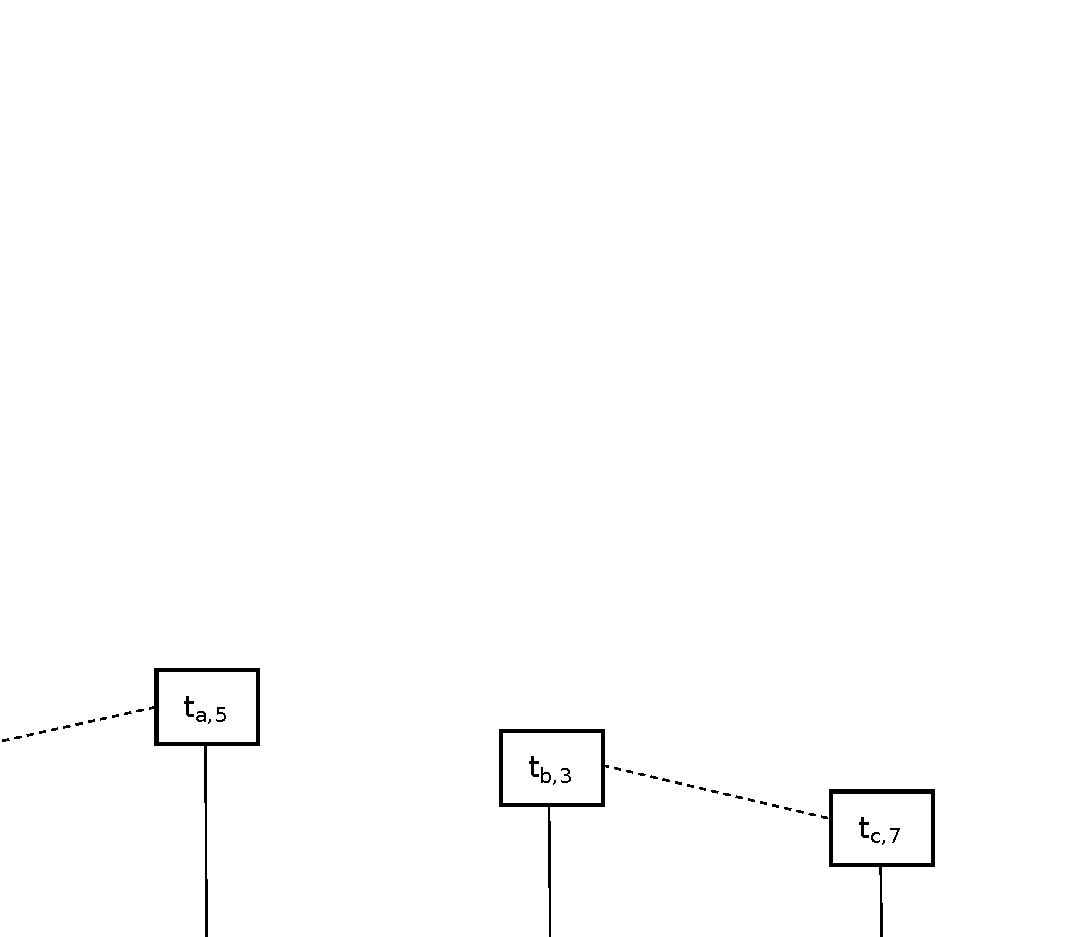
\includegraphics[trim={0 0 0 11cm}, clip, width=1.0\textwidth]{trustchain-1}
    \centering
    \caption{We begin in a state where some facilitators $\F_{r-2}$ just agreed on the consensus result $\C_{r-1}$ but have not yet propogated it yet.}
    \label{fig:trustchain-1}
\end{figure}

\begin{figure}[htb]
    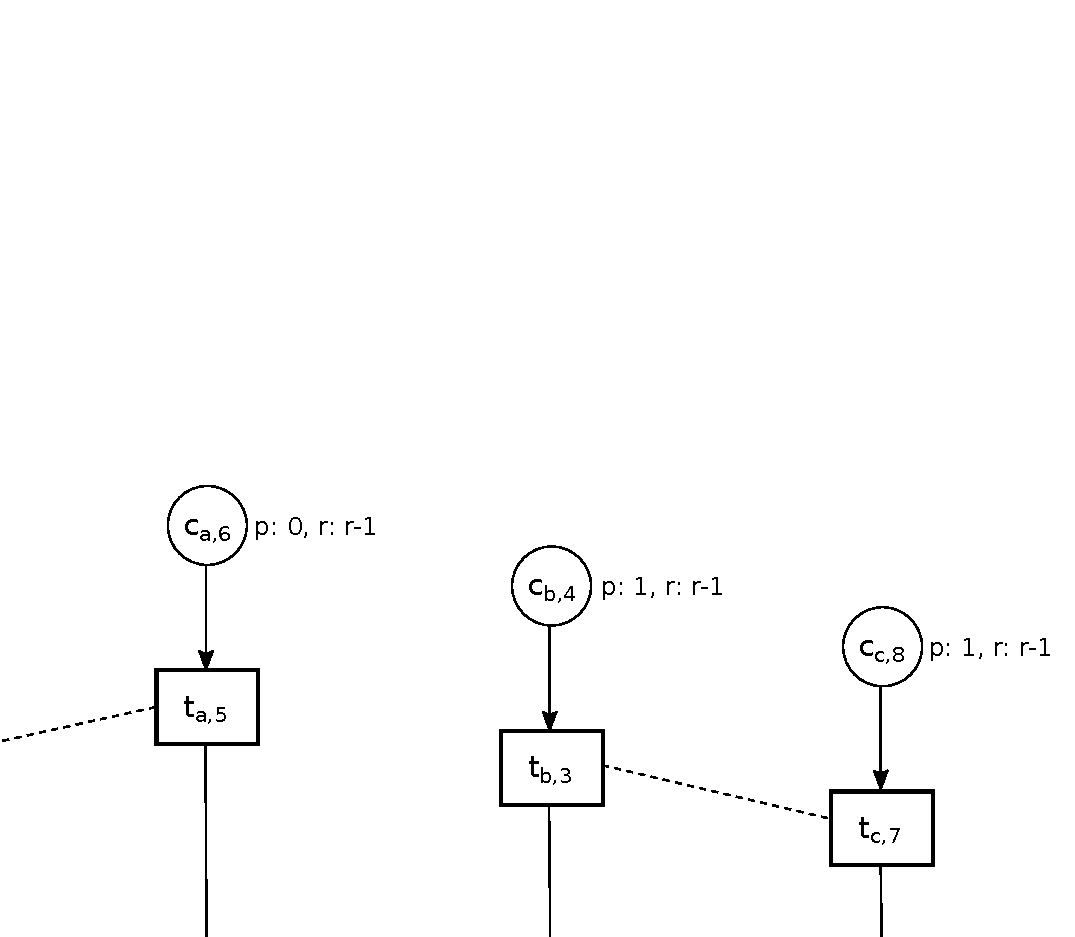
\includegraphics[trim={0 0 0 8cm}, clip, width=1.0\textwidth]{trustchain-2}
    \centering
    \caption{The facilitators propogates $\C_{r-1}$. Upon receiving it, the nodes perform two tasks;
    (1) elect new facilitators $\F_{r-1}$ by selecting the first $n$ nodes ordered by $\textsf{H}(\C_{r-1} || pk)$,
    and (2) create new CP blocks---$c_{a, 6}, c_{b, 4}$ and $c_{c, 8}$.
    $\textsf{H}(\cdot)$ is a cryptographically secure hash function and $pk$ is the public key of the respective node.}
    \label{fig:trustchain-2}
\end{figure}

\begin{figure}
    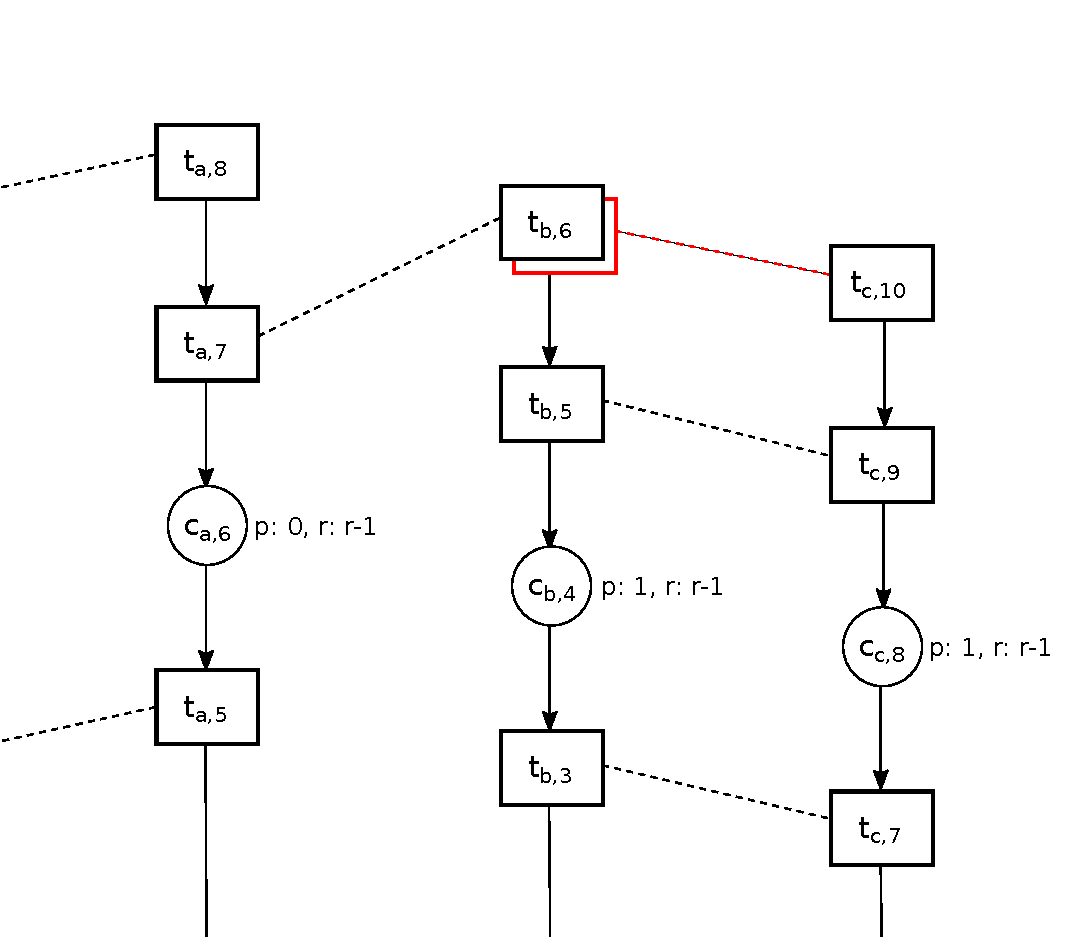
\includegraphics[trim={0 0 0 2cm}, clip, width=1.0\textwidth]{trustchain-3}
    \centering
    \caption{Nodes now send their new CP blocks to the new facilitators $\F_{r-1}$.
    While $\F_{r-1}$ is trying to reach consensus on a set of CP blocks,
    nodes carry on making transactions as usual (concurrently).
    We remark that the to-be-agreed consensus result $\C_r$ is created using CP blocks from the previous round---$c_{a, 6}, c_{b, 4}$ and $c_{c, 8}$.
    }
    \label{fig:trustchain-3}
\end{figure}

\begin{figure}
    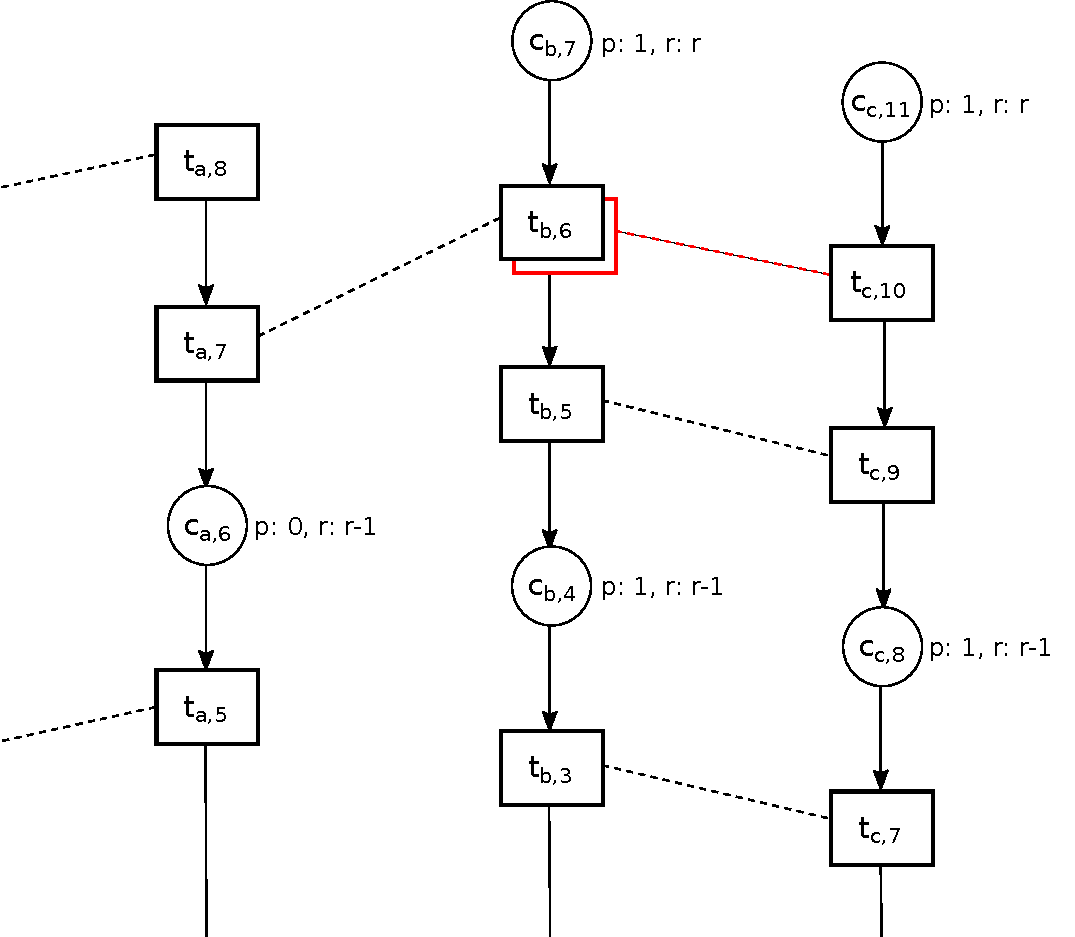
\includegraphics[width=1.0\textwidth]{trustchain-4}
    \centering
    \caption{Finally, when $\F_{r-1}$ decides on $\C_r$ (which should contain $c_{a, 6}, c_{b, 4}$ and $c_{c, 8}$) and disseminates it.
    Nodes compute new facilitators $\F_{r}$ and create new CP blocks.}
    \label{fig:trustchain-4}
\end{figure}

\end{document}

